\documentclass[a4paper,10pt,BCOR10mm,oneside,headsepline]{scrartcl}
\usepackage{amsmath, mathtools}
\usepackage[ngerman]{babel}
\usepackage[utf8]{inputenc}
\usepackage{graphicx}
\usepackage{float}

\usepackage{typearea, url}
\areaset{17cm}{26cm}
\setlength{\topmargin}{-1cm}
\usepackage{scrlayer-scrpage}
\pagestyle{scrheadings}

\usepackage[T1]{fontenc}
\usepackage{beramono}
\usepackage{listings}
\usepackage[usenames,dvipsnames]{xcolor}


%%
%% Julia definition (c) 2014 Jubobs
%%
\lstdefinelanguage{Julia}%
  {morekeywords={abstract,break,case,catch,const,continue,do,else,elseif,%
      end,export,false,for,function,immutable,import,importall,if,in,%
      macro,module,otherwise,quote,return,switch,true,try,type,typealias,%
      using,while},%
   sensitive=true,%
   alsoother={$},%
   morecomment=[l]\#,%
   morecomment=[n]{\#=}{=\#},%
   morestring=[s]{"}{"},%
   morestring=[m]{'}{'},%
}[keywords,comments,strings]%

\lstset{%
    language         = Julia,
    basicstyle       = \ttfamily,
    keywordstyle     = \bfseries\color{blue},
    stringstyle      = \color{magenta},
    commentstyle     = \color{ForestGreen},
    showstringspaces = false,
}



\ihead{HW1: CIS 410/510, Computational Science, Fall 2022}
\ohead{\pagemark}
\chead{}
\cfoot{}

%%%%%%%%%%%%%%%%%%%%%%%%%%%%%%%%%%%%%%%%%%%%%%%%%%%%%%%%%%%%
%% Beginning of questionnaire command definitions %%
%%%%%%%%%%%%%%%%%%%%%%%%%%%%%%%%%%%%%%%%%%%%%%%%%%%%%%%%%%%%
%%
%% 2010, 2012 by Sven Hartenstein
%% mail@svenhartenstein.de
%% http://www.svenhartenstein.de
%%
%% Please be warned that this is NOT a full-featured framework for
%% creating (all sorts of) questionnaires. Rather, it is a small
%% collection of LaTeX commands that I found useful when creating a
%% questionnaire. Feel free to copy and adjust any parts you like.
%% Most probably, you will want to change the commands, so that they
%% fit your taste.
%%
%% Also note that I am not a LaTeX expert! Things can very likely be
%% done much more elegant than I was able to. If you have suggestions
%% about what can be improved please send me an email. I intend to
%% add good tipps to my website and to name contributers of course.
%%
%% 10/2012: Thanks to karathan for the suggestion to put \noindent
%% before \rule!

%% \Qq = Questionaire question. Oh, this is just too simple. It helps
%% making it easy to globally change the appearance of questions.
\newcommand{\Qq}[1]{\textbf{#1}}

%% \QO = Circle or box to be ticked. Used both by direct call and by
%% \Qrating and \Qlist.
\newcommand{\QO}{$\Box$}% or: $\ocircle$

%% \Qrating = Automatically create a rating scale with NUM steps, like
%% this: 0--0--0--0--0.
\newcounter{qr}
\newcommand{\Qrating}[1]{\QO\forloop{qr}{1}{\value{qr} < #1}{---\QO}}

%% \Qline = Again, this is very simple. It helps setting the line
%% thickness globally. Used both by direct call and by \Qlines.
\newcommand{\Qline}[1]{\noindent\rule{#1}{0.6pt}}

%% \Qlines = Insert NUM lines with width=\linewith. You can change the
%% \vskip value to adjust the spacing.
\newcounter{ql}
\newcommand{\Qlines}[1]{\forloop{ql}{0}{\value{ql}<#1}{\vskip0em\Qline{\linewidth}}}

%% \Qlist = This is an environment very similar to itemize but with
%% \QO in front of each list item. Useful for classical multiple
%% choice. Change leftmargin and topsep accourding to your taste.
\newenvironment{Qlist}{%
\renewcommand{\labelitemi}{\QO}
\begin{itemize}[leftmargin=1.5em,topsep=-.5em]
}{%
\end{itemize}
}

%% \Qtab = A "tabulator simulation". The first argument is the
%% distance from the left margin. The second argument is content which
%% is indented within the current row.
\newlength{\qt}
\newcommand{\Qtab}[2]{
\setlength{\qt}{\linewidth}
\addtolength{\qt}{-#1}
\hfill\parbox[t]{\qt}{\raggedright #2}
}

%% \Qitem = Item with automatic numbering. The first optional argument
%% can be used to create sub-items like 2a, 2b, 2c, ... The item
%% number is increased if the first argument is omitted or equals 'a'.
%% You will have to adjust this if you prefer a different numbering
%% scheme. Adjust topsep and leftmargin as needed.
\newcounter{itemnummer}
\newcommand{\Qitem}[2][]{% #1 optional, #2 notwendig
\ifthenelse{\equal{#1}{}}{\stepcounter{itemnummer}}{}
\ifthenelse{\equal{#1}{a}}{\stepcounter{itemnummer}}{}
\begin{enumerate}[topsep=2pt,leftmargin=2.8em]
\item[\textbf{\arabic{itemnummer}#1.}] #2
\end{enumerate}
}

%% \QItem = Like \Qitem but with alternating background color. This
%% might be error prone as I hard-coded some lengths (-5.25pt and
%% -3pt)! I do not yet understand why I need them.
\definecolor{bgodd}{rgb}{0.8,0.8,0.8}
\definecolor{bgeven}{rgb}{0.9,0.9,0.9}
\newcounter{itemoddeven}
\newlength{\gb}
\newcommand{\QItem}[2][]{% #1 optional, #2 notwendig
\setlength{\gb}{\linewidth}
\addtolength{\gb}{-5.25pt}
\ifthenelse{\equal{\value{itemoddeven}}{0}}{%
\noindent\colorbox{bgeven}{\hskip-3pt\begin{minipage}{\gb}\Qitem[#1]{#2}\end{minipage}}%
\stepcounter{itemoddeven}%
}{%
\noindent\colorbox{bgodd}{\hskip-3pt\begin{minipage}{\gb}\Qitem[#1]{#2}\end{minipage}}%
\setcounter{itemoddeven}{0}%
}
}

%%%%%%%%%%%%%%%%%%%%%%%%%%%%%%%%%%%%%%%%%%%%%%%%%%%%%%%%%%%%
%% End of questionnaire command definitions %%
%%%%%%%%%%%%%%%%%%%%%%%%%%%%%%%%%%%%%%%%%%%%%%%%%%%%%%%%%%%%

\begin{document}

\begin{center}
\textbf{\large CIS 410/510 HW 2 - Brett Sumser%\footnote{Subject to change}
}
\end{center}\vskip1em

For the first part of this assignment, we have to implement the conjugate gradient descent algorithm. This algorithm is used
to find a numerical solution for a system of linear equations where the matrix is positive definite. To check my implement for correctness,
I implemented a test function that ran the algorithm on a small system where the solution was known.

Here are the functions I was able to successfully implement:

\begin{itemize}
  \item conj grad(A, x, b, $\epsilon$, item max) - This is my implementation of the conjugate gradient algorithm.
    It takes a positive definite matrix A, an initial guess vector x, a tolerance \epsilon and a max iteration as arguments.

  \item conj grad test() - This is a test implementation of the conjugate gradient algorithm, but it solves a known system with a size
    N = 2. It calls the above function and compares the result against the known solution. This is how I checked that my implementation
    was working correctly.

  \item err R(A, x, b) - This function calculates the relative error, using a helper magnitude function to calculate:

    $err_R = \frac{||Ax - b||}{||x||}$

  \item var set(N) - This function sets the variables needed for the gradient algorithm, taking a size N and setting up the required vectors
    and matrix.

  \item magnitude(x) -This function takes a vector x and performs the 2-norm calculation.

\end{itemize}

From the below figure, it can be seen that up to $N = 1000$, the time is fairly consistent. But once you get up to $N = 10000$, the amount
of time it takes for the algorithm to run increases by roughly 40x! I am not sure if I calculated my residuals correctly, but it seems like they grow
cyclicly.

\begin{figure}[h]
\centering
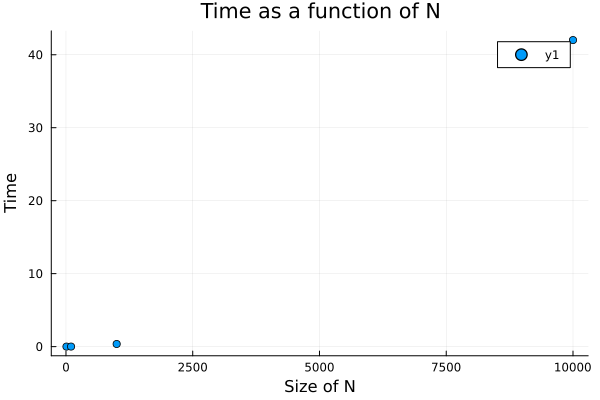
\includegraphics[scale=0.75]{testPlot.png}
\end{figure}

\begin{figure}[h]
\centering
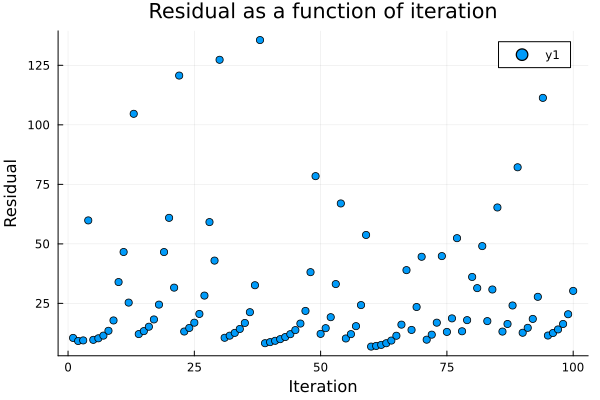
\includegraphics[scale=0.75]{testPlotNew.png}
\end{figure}

\newpage

For the second part of the assignment, I struggled with modifying forwards euler into a backwards implmentation. Admittedly, I spent most of the
time for the assignment working on the conjugate gradient, and might have overestimated how easy the second part would be.
I was able to plot a line for the function $g(x) = 17*e^(-3t)$, and it shoes that the values seem to converge appropriatly. I also was not sure
how to plot a stable time step. I ended up using $\deltat = 0.5$.

\begin{figure}[h]
\centering
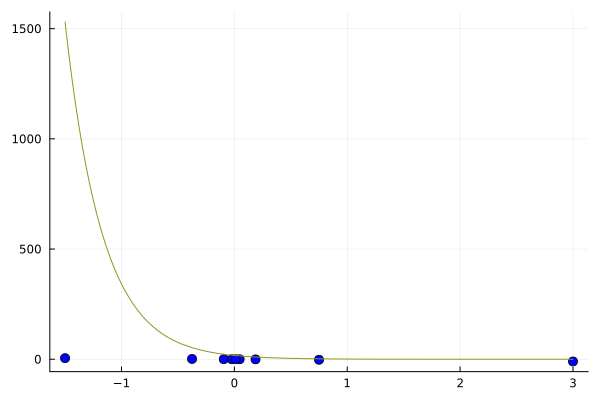
\includegraphics[scale=0.75]{testPlotEulerForward.png}
\end{figure}

\newpage

\begin{lstlisting}

using Plots # add Plots.jl from the package manager if you have not already done so.
using Printf # for formatting text output

# HW 1 starting script (if you want): contains function computeLU() - to compute an LU-factorization of square
# matrix A, namely, A = LU, where L and U are lower and upper triangular matrices.

#-------------------------HOMEWORK 2 FUNCTIONS------------------------------------------#
#---------------------------------------------------------------------------------------#
"""
    conj_grad(A, x, b, ϵ, iter_max)

Function that performs conjugate gradient algorithm given:
    A - positive definite matrix
    x_0 - initial guess
    ϵ - tolerance
    iter_max - maximum number of iterations

Returns approximate solution to Ax = b, where relative err_R <= ϵ
"""
function conj_grad(A, x, b, ϵ, iter_max)
    res_i = []
    N = size(A, 1)
    r = Matrix{Float64}(undef, N, 1)
    r .= 0
    r = r[:]

    α = Matrix{Float64}(undef, N, 1)
    α .= 0
    α = α[:]

    β = Matrix{Float64}(undef, N, 1)
    β .= 0
    β = β[:]

    p = Matrix{Float64}(undef, N, 1)
    p .= 0
    p = p[:]

    new_r = Matrix{Float64}(undef, 2, 1)
    new_r .= 0
    new_r = r[:]

    new_x = 0

    new_p = Matrix{Float64}(undef, 2, 1)
    new_p .= 0
    new_p = r[:]

    r = b - A * x
    p .= r

    for i = 1:iter_max # march across columns
        α = (r'*r) ./ (p'*A*p)
        new_x = x + α .* p
        x = new_x
        new_r .= r - α .* A * p
        β = (new_r' * new_r) ./ (r' * r)
        if (err_R(A,x,b) <= ϵ)
            display("converged")
            return new_x
        end
        push!(res_i, (magnitude(A * x - b)))
        r = new_r
        new_p .= new_r + β .* p
        p = new_p
    end

    return (new_x, res_i)
end

"""
    conj_grad_test()

This is a test function for the conjugate gradient algorithm.
It solves a simple Ax = b using matrix and vectors of size 2 with a known solution
"""
function conj_grad_test()
    N = 2
    B = rand(N,N)

    b = rand(N,1)
    b = b[:]

    A = Matrix{Float64}(undef, 2, 2)
    A .= [4 1;1 3]
    display(A)

    x = Matrix{Float64}(undef, 2, 1)
    x .= 0
    x = x[:]
    x = [2 1]
    x = vec(x)
    display(x)

    b = Matrix{Float64}(undef, 2, 1)
    b .= 0
    b = [:]
    b = [1 2]
    b = vec(b)
    display(b)

    r = Matrix{Float64}(undef, 2, 1)
    r .= 0
    r = r[:]
    display(r)

    p = Matrix{Float64}(undef, 2, 1)
    p .= 0

    ϵ = 10^-6
    iter_max = 2

    x = conj_grad(A, x, b, ϵ, iter_max)
    return x

end

"""
    err_R(A, x, b)

Function that calculates the relative error based on formula in assignment
"""
function err_R(A, x, b)
    err_r = magnitude(A * x - b) / magnitude(x)
    return err_r
end

"""
    var_set(N)

Function that prepares variables for conjugate gradient algorithm.
Takes parameter N for size of matrix/vectors. Returns:
    A - random matrix of size N made using A = I +B^T B, where I is the identity matrix and B is a rand(N,N) matrix
    b - random vector of size N
    x - 0 vector for initial guess
"""
function var_set(N)
    ϵ = 10^-4
    iter_max = 100
    A = Matrix{Float64}(undef, N, N)

    B = rand(N,N)
    b = rand(N,1)
    b = b[:]

    x = rand(N,1)
    x .= 0
    x = x[:]

    I = Matrix{Float64}(undef, N, N)
    I .= 0

    for i = 1:N
        I[i,i] = 1
    end
    A .= I .+ B'B

    return (A, b, x, ϵ, iter_max)
end

"""
    magnitude(x)

Performs magnitude calculation of vector
"""
function magnitude(x)
    N = size(x, 1)
    sum = 0
    mag = 0
    for i = 1:N
        sum += (x[i])^2
    end
    mag = sqrt(sum)
    return mag
end
#-------------------------END HOMEWORK 2 FUNCTIONS------------------------------------------#
#-------------------------------------------------------------------------------------------#

#-------------------------HOMEWORK 1 FUNCTIONS------------------------------------------#
#---------------------------------------------------------------------------------------#
"""
    computeLU(A)
Compute and return LU factorization `LU = A` of square matrix `A`.
Might not work on all matrices, since no pivoting is done!
# Examples (don't need examples, but fine to include)
'''
julia> A = [6 -2 2;12 -8 6;3 -13 3]
3×3 Array{Int64,2}:
  6   -2  2
 12   -8  6
  3  -13  3
julia> (L, U) = computeLU(A)
([1.0 0.0 0.0; 2.0 1.0 0.0; 0.5 3.0 1.0], [6.0 -2.0 2.0; 0.0 -4.0 2.0; 0.0 0.0 -4.0])
julia> norm(A - L*U)
0.0
'''
"""
function computeLU(A)

    N = size(A)[1]

    #Id = Matrix{Float64}(I, N, N) # N x N identity matrix
    Id = create_identity(N)

    L = copy(Id)   # initialize
    U = copy(Id)   # initialize
    Ã  = copy(A) # initialize. Ã corresponds to A as it goes under elimination stages

    for k = 1:N-1 # march across columns

        (Lk, Lk_inv) = compute_Lk(Ã, k)

        Ã .= Lk * Ã
        L .= L * Lk_inv

    end

    U .= Ã

    return (L, U)

end


"""
    compute_Lk(A, k)
Compute Lk and its inverse from A, assuming first k-1 columns have undergone elimination.
"""
function compute_Lk(A, k)


    N = size(A)[1]

    Lk = create_identity(N) # Matrix{Float64}(I, N, N)       # initialize as identity matrix
    Lk_inv = create_identity(N)# Matrix{Float64}(I, N, N)   # initialize as identity matrix

    # now modify column k, strictly below diagonal (i = k+1:N)
    for i = k+1:N
        Lk[i,k] = -A[i,k] / A[k,k]    # fill me in (compute elimination factors)
        Lk_inv[i,k] = A[i,k] / A[k,k]  # fill me in (compute elimination factors)
    end

    return (Lk, Lk_inv)

end

"""
    create_identity(N)
Given integer N, constructs a square identity matrix of size N.
"""
function create_identity(N)

    I = Matrix{Float64}(undef, N, N)
    I .= 0

    for i = 1:N
        I[i, i] = 1
    end

    return I
end

"""
    find_pivot(A, k)

Given matrix A and column k, find largest element in that column. Uses built in method findmax(A[]),
where A[] is the proper slice of the matrix for the column we need. findmax() returns the value of the max found,
and a Cartesian Coordinate pair for the index of the element.

julia> A .= [6 -2 2;12 -8 6;3 -13 3]
3×3 Matrix{Float64}:
  6.0   -2.0  2.0
 12.0   -8.0  6.0
  3.0  -13.0  3.0

julia> A[:,1:1]
3×1 Matrix{Float64}:
  6.0
 12.0
  3.0

julia> A[:,2:2]
3×1 Matrix{Float64}:
  -2.0
  -8.0
 -13.0
"""
function find_pivot(A, k)
    return (value, index) = findmax(A[:,k:k])
end

"""
    swap(L, j, k)

Function that swaps rows j and k in all columns from 1:k-1 in matrix L by constructing the proper
permutation matrix.
"""
function swap(L, j, k)
    print("swap called")
    N = size(L)[1]
    I = Matrix{Float64}(undef, N, N)
    I .= 0

    for i = 1:N
        I[i,i] = 1
    end

    for i = 1:N
        I[j,i], I[k,i] = I[k,i], I[j,i]
    end

    L .= I * L

    return L
end

"""
    luDoolittleDecomp(A, N)

Function that performs an LU decomposition using the doolittle algorithm.
"""
function luDoolittleDecomp(A,N)
    U = Matrix{Float64}(undef, N, N)
    U .= 0

    L = Matrix{Float64}(undef, N, N)
    L .= 0

    for i = 1:N
        for k = i:N
            sum = 0
            for j = 1:i
                sum += (L[i,j] * U[j,k])

            end
            U[i,k] = A[i,k] - sum
        end
        for k = i:N
            if (i == k)
                L[i,i] = 1
            else
                sum = 0
                for j = 1:i
                    sum += (L[k,j] * U[j,i])
                end
                L[k,i] = (A[k,i] - sum) / U[i,i]
            end
        end
    end
    #display(U)
    #display(L)
    return(L,U)
end

"""
    LUPsolve(A)

Function that solves Ax=b by computing LUP-factorization and performs forward/backward substitution.
"""
function LUPsolve(A, b)
    # test matrix to check for accuracy in solving
    #L = Matrix{Float64}(undef, 3, 3)
    #L .= [1 0 0;4 1 0;4 0.5 1]
    #U = Matrix{Float64}(undef, 3, 3)
    #U .= [1 2 2;0 -4 -6;0 0 -1]

    #size of matrix working
    N = size(A)[1]

    (L,U) = luDoolittleDecomp(A,N)
    #display(U)
    #display(L)

    y = forward_sub(L, b)
    x = backward_sub(U, y)

    #display(x)
    return x
end

"""
    forward_sub(L, b)

Give lower triangular matrix L and vector b, perform the forward substitution to solve linear system Lx = b
"""
function forward_sub(L, b)
    N = size(L)[1]
    x = similar(L)
    x .= 0

    for i = 1:N
        temp = b[i]
        for j = 1:i-1
            temp -= L[i,j] * x[j]
        end
        x[i] = temp / L[i,i]
    end
    return x
end


"""
    backward_sub(U, b)

Give upper triangular matrix U and vector b, perform the forward substitution to solve linear system Ux = b
(Backward version of forward substitution)
"""
function backward_sub(U, b)
    N = size(U)[1]
    x = similar(U)
    x .= 0

    for i = N:-1:1
        temp = b[i]
        for j = i+1:N
            temp -= U[i,j] * x[j]
        end
        x[i] = temp / U[i,i]
    end
    return x
end

#-------------------------END HOMEWORK 1 FUNCTIONS------------------------------------------#
#-------------------------------------------------------------------------------------------#

"""
    main()

Main function to perform conjugate gradient at sizes N = 10, 100, 1000, 10000
Also outputs a plot with time as a function of N
"""
function main()
    y_time = []
    testSizes = [10, 100, 1000]
    @printf("starting loop for values")
    for i = 1:size(testSizes,1)
        (A, b, x, ϵ, iter_max) = var_set(testSizes[i])
        temp = @timed (x, res_i) = conj_grad(A, x, b, ϵ, iter_max)
        push!(y_time, temp[2])
        @printf("done at N = %d\n", testSizes[i])
    end
    @printf("done\n")
    res_i = []
    step = rand(100,1)
    step .= 0
    step = step[:]
    for i = 1:100
        step[i] = i
    end
    (A, b, x, ϵ, iter_max) = var_set(1000)
    (x, res_i) = conj_grad(A, x, b, ϵ, iter_max)
    scatter(step, res_i, xlabel="Iteration", ylabel="Residual", title = "Residual as a function of iteration")
    savefig("testPlotNew.png")
end

main()

#b = rand(3, 1)
#
#(L, U) = computeLU(A)
#@assert A*x[iter_max] ≈ b

using Plots

# write forward Euler for the IVP system y' = f(t, y)
# where y is a vector in R^n (i.e. has n components)

function f(t,y)
    return -3 * y
end

"""
    my_forward_euler(t0, Tf, Δt, y0, f)

Function to perform the forwards euler algorithm.
"""
function my_forward_euler(t0, Tf, Δt, y0, f)

    # y0 has N components
    N = size(y0)

    M = Integer(Tf/Δt)  # M+1 total temporal nodes

    t = Vector{Float64}(undef, M+1)
    y = Matrix{Float64}(undef, N, M+1)

    # fill in the initial condition:
    t[1] = t0
    y[:, 1] = y0

    for n = 1:M # take N time steps
        y[:, n+1] = y[:, n] + Δt*f(t[n],y[:, n])
        t[n+1] = t[n] + Δt
    end

    return (t, y)
end


"""
    my_backward_euler(t0, Tf, Δt, y0, f)

Function to perform backwards euler algorithm.
"""
function my_backward_euler(t0, Tf, Δt, y0, f)
    # y0 has N components
    N = size(y0)

    M = Integer(Tf/Δt)  # M+1 total temporal nodes

    t = Vector{Float64}(undef, M+1)
    y = Matrix{Float64}(undef, N, M+1)

    # fill in the initial condition:
    t[1] = t0
    y[:, 1] = y0

    for n = 1:M # take N time steps
        y[:, n+1] = y[:, n] + Δt*f(t[n+1],y[:, n+1])
        t[n+1] = t[n] + Δt
    end
    scatter(t, y, xlabel="time", ylabel="Y-value", title = "Y values as function of time step")
    savefig("testPlotEuler.png")

    return (t, y)
end


# Write forward Euler to solve the linear system IVP:
# y' = Ay + b on 0 ≤ t ≤ Tf
# with initial y0

# Do this on particular example, where A = [-3 13; -5 -1]
# y0 = [3; -10]

t0 = 0
y0 = [3; -10]

#A = [-3 13;-5 -1]

Tf = 4
Δt = 0.5

N = Integer(Tf/Δt) # N+1 total temporal nodes


y = Matrix{Float64}(undef, 2, N+1)
t = Vector{Float64}(undef, N+1)
t[1] = 0
# fill in initial condition:
y[:, 1] = y0


for n = 1:N  # take N time steps
    y[:, n+1] = y[:, n] + Δt*-3*y[:, n]  # Forward Euler
    t[n+1] = t[n] + Δt
end


#plot(t, y[1, :])  # plot first component of solution vector
#plot!(t, y[2, :])  # plot second component

# plot initial condition:
p = plot([y[1, 1]], [y[2, 1]], marker=(:circle,5), color = :blue, legend = false)

g(x) = 17*2.71828^(-3x)

for n = 2:N+1
    p = plot!([y[1, n]], [y[2, n]], marker=(:circle,5), color = :blue, legend = false)
    display(p)
    sleep(1)
end
plot!(g)
savefig("testPlotEulerForward.png")

my_backward_euler(t0, Tf, Δt, y0, f)

\end{lstlisting}
\end{document}
